\begin{prob}[3.1]
  Consider the optimization problem
  \begin{eqnarray*}
    \mbox{minimize} & f_{0}(x_{1}, x_{2})\\
    & 2 x_{1} + x_{2} \geq 1\\
    \mbox{subject to} & x_{1} + 3x_{2} \geq 1\\
    & x_{1} \geq 0,x_{2} \geq 0
  \end{eqnarray*}

  Make a sketch of the feasible set. For each of the following functions, give
  the optimal set and the optimal value. Then use CVX to verify the optimal
  values you obtained.
\end{prob}
 \begin{enumerate}[label=(\alph*)]
  \item{$f_{0}(x_{1},x_{2}) = x_{1} + x_{2}$
    \begin{proof}[\sol]
      The solution would be $x* = \left ( \dfrac{2}{5},\dfrac{1}{5}\right )$
      %\mylisting{\src{h3q1a.asv}}
      \verbatiminput{source/h3q1a.m}
      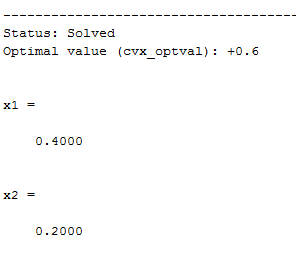
\includegraphics[width=4cm]{source/h3q1a}
    \end{proof}    
  }
    \newpage
  \item{$f_{0}(x_{1},x_{2}) = -x_{1} - x_{2}$
    \begin{proof}[\sol]
      This is unbounded
      \verbatiminput{source/h3q1b.m}
      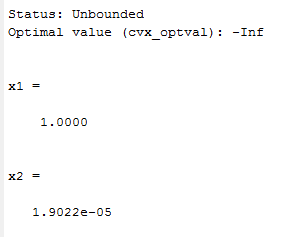
\includegraphics{source/h3q1b}
    \end{proof}
  }
    \newpage
   \item{$f_{0}(x_{1},x_{2}) = x_{1}$
     \begin{proof}[\sol] Since, this one only depends on $x_{1}$, then our
       solution is $X = \{(0, x_{2}) | x_{2} \geq 1\}$
       \verbatiminput{source/h3q1c.m}
       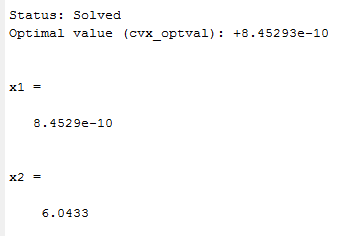
\includegraphics{source/h3q1c}
       Here, we notice that the value for $x_{1}$ is small, thus essentially 0.
    \end{proof}
   }
     \newpage
   \item{$f_{0}(x_{1},x_{2}) = \max\{x_{1}, x_{2}\}$
     \begin{proof}[\sol]
       The solution is $x* = \left ( \dfrac{1}{3}, \dfrac{1}{3} \right )$
       \verbatiminput{source/h3q1d.m}
      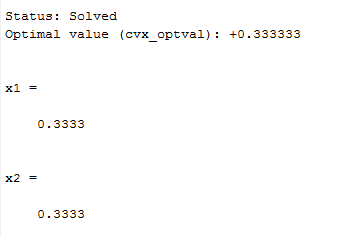
\includegraphics{source/h3q1d}
    \end{proof}
   }
     \newpage
   \item{$f_{0}(x_{1},x_{2}) = x_{1}^{2} + 9x_{2}^{2}$
     \begin{proof}[\sol]
       The solution is $x* = \left ( \dfrac{1}{2}, \dfrac{1}{6} \right )$
       \verbatiminput{source/h3q1e.m}
      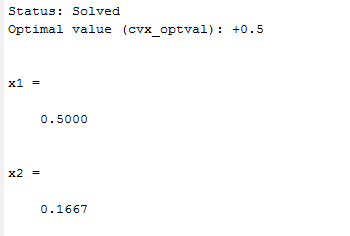
\includegraphics{source/h3q1e}
    \end{proof}
   }
  \end{enumerate}
